\documentclass[12pt]{article}
\renewcommand{\familydefault}{\sfdefault}

\usepackage[margin=0.5in]{geometry}

\usepackage{scrextend}


\usepackage[capitalise]{cleveref}

%\usepackage{umuphys}            % Local umu-physics firstpage style
\usepackage{graphicx}         % To include graphics
\usepackage{tikz}

\usepackage{tabularx}

\usepackage{booktabs}
\usepackage{multirow}
\usepackage{colortbl}
\setlength{\tabcolsep}{2pt}

\author{xxAuthor Namexx}
\title{UN Sustainable Development Goals For xxMSAxx}

% Optional commands: \email and \bottomtext

\newcommand{\allgoalwidth}{0.046\linewidth}

\begin{document}
%\maketitle

\begin{figure}[ht]
	\centering
	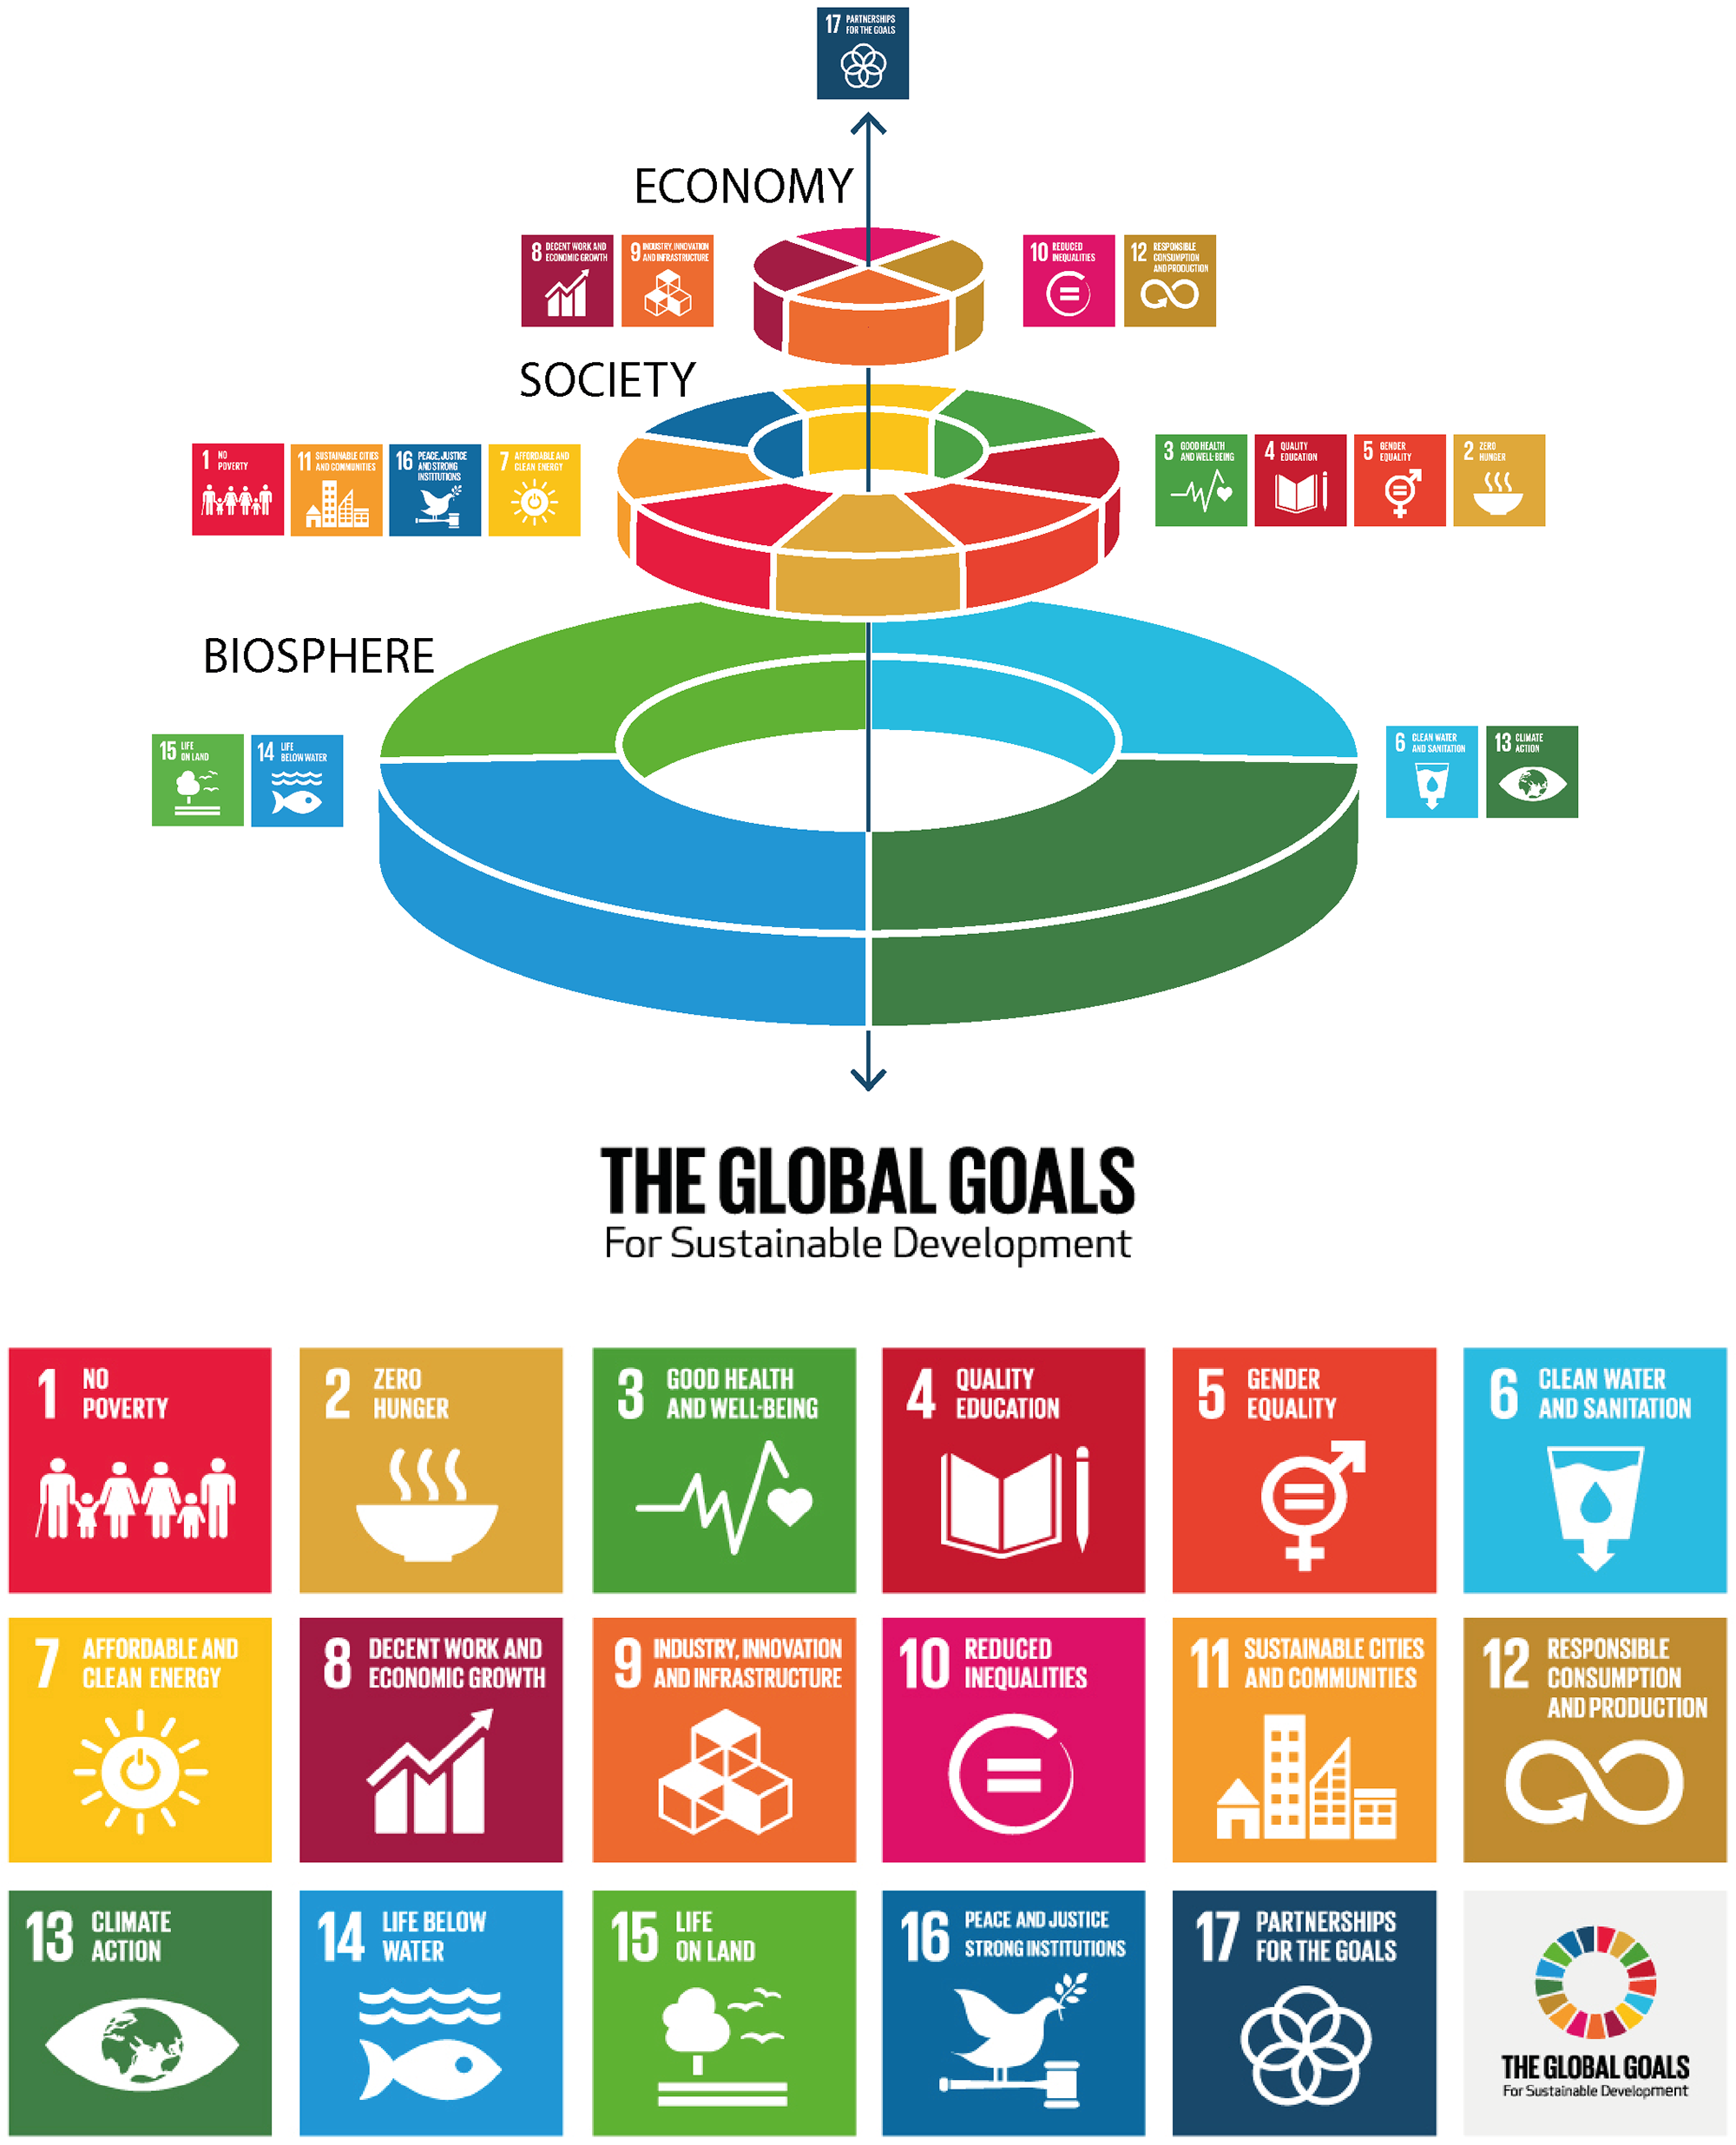
\includegraphics[width=\linewidth]{../figs/pyramid-figure4.png}
	\label{fig:cover}
\end{figure}

\clearpage

\maketitle

\section*{Summary}
A summary statement of the goals goes here

\cref{tab:summary} shows a summary of where we stand as of 20XX. The xxMSAxx ranks xxRANKxx out of 105 U.S. metropolitan areas, as measured by these 17 goals, with an average score of xxAVGSCORExx\% across all. Two of the goals, 14 - Life Below Water and 17 - Partnerships for the Goals, are not being measured, for any city, because there are no currently measurable data for them. Other data gaps exist and are detailed in \cref{sec:datagap}. Below each top-level goal are the measurable targets. The normalized value of how close our community comes to these targets determines our score, and the average of these scores is the score for the goal.

TODO THIS SUMMARY TABLE IS NOT COMPLETE (NORM SCORE VS RAW)

%1/17 is 0.0588
%1/18 is 0.0556

%do the tabsep before the first colum and all the rest
\input{summary-table}

The remainder of this document details the performance of our community on the individual targets at the rates/units described.


\clearpage
%%%%%%%%%%%%%%%%%%%%%%%%%%%%%%%%%%%%%%%%%%%%%%
\section{No Poverty}  %nothing yet
%\begin{figure}[ht]
%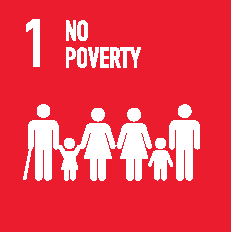
\includegraphics[width=5em]{./figs/Goal1.pdf}
%\end{figure}
\input{./tab-sdg1}
\input{./sec-sdg1}

%%%%%%%%%%%%%%%%%%%%%%%%%%%%%%%%%%%%%%%%%%%%%%
\section{Zero Hunger}
\input{./tab-sdg2}
\input{./sec-sdg2}

%%%%%%%%%%%%%%%%%%%%%%%%%%%%%%%%%%%%%%%%%%%%%%
\section{Good Health and Well Being}
\input{./tab-sdg3}
\input{./sec-sdg3}

%%%%%%%%%%%%%%%%%%%%%%%%%%%%%%%%%%%%%%%%%%%%%%
\section{Quality Education}
\input{./tab-sdg4}
\input{./sec-sdg4}

%%%%%%%%%%%%%%%%%%%%%%%%%%%%%%%%%%%%%%%%%%%%%%
\section{Gender Equality}
\input{./tab-sdg5}
\input{./sec-sdg5}

%%%%%%%%%%%%%%%%%%%%%%%%%%%%%%%%%%%%%%%%%%%%%%
\section{Clean Water and Sanitation}
\input{./tab-sdg6}
\input{./sec-sdg6}

%%%%%%%%%%%%%%%%%%%%%%%%%%%%%%%%%%%%%%%%%%%%%%
\section{Affordable and Clean Energy}
\input{./tab-sdg7}
\input{./sec-sdg7}

%%%%%%%%%%%%%%%%%%%%%%%%%%%%%%%%%%%%%%%%%%%%%%
\section{Decent Work and Economic Growth}
\input{./tab-sdg8}
\input{./sec-sdg8}

%%%%%%%%%%%%%%%%%%%%%%%%%%%%%%%%%%%%%%%%%%%%%%
\section{Industry, Innovation, and Infrastructure}
\input{./tab-sdg9}
\input{./sec-sdg9}

%%%%%%%%%%%%%%%%%%%%%%%%%%%%%%%%%%%%%%%%%%%%%%
\section{Reduced Inequalities}
\input{./tab-sdg10}
\input{./sec-sdg10}

%%%%%%%%%%%%%%%%%%%%%%%%%%%%%%%%%%%%%%%%%%%%%%
\section{Sustainable Cities and Communities}
\input{./tab-sdg11}
\input{./sec-sdg11}

%%%%%%%%%%%%%%%%%%%%%%%%%%%%%%%%%%%%%%%%%%%%%%
\section{Responsible Consumption and Production}
\input{./tab-sdg12}
\input{./sec-sdg12}

%%%%%%%%%%%%%%%%%%%%%%%%%%%%%%%%%%%%%%%%%%%%%%
\section{Climate Action}
\input{./tab-sdg13}
\input{./sec-sdg13}

%%%%%%%%%%%%%%%%%%%%%%%%%%%%%%%%%%%%%%%%%%%%%%
\section{Life Below Water}
There are currently no measures in place to score this Goal. See \Cref{sec:datagap}.
\clearpage

%%%%%%%%%%%%%%%%%%%%%%%%%%%%%%%%%%%%%%%%%%%%%%
\section{Life On Land}
\input{./tab-sdg15}
\input{./sec-sdg15}

%%%%%%%%%%%%%%%%%%%%%%%%%%%%%%%%%%%%%%%%%%%%%%
\section{Peace, Justice, and Strong Institutions}
\input{./tab-sdg16}
\input{./sec-sdg16}

%%%%%%%%%%%%%%%%%%%%%%%%%%%%%%%%%%%%%%%%%%%%%%
\section{Partnerships for the Goals}
There are currently no measures  in place to score this Goal. See \Cref{sec:datagap}.
\clearpage

%%%%%%%%%%%%%%%%%%%%%%%%%%%%%%%%%%%%%%%%%%%%%%
\section{Data gaps}\label{sec:datagap}
There are multiple data gaps in each goal, research is on-going to close these gaps and develop repeatable, scientific measurements of these items (TAD-TODO).

\end{document}